\documentclass[11pt,a4paper]{article}
\usepackage[utf8]{inputenc}
\usepackage[a4paper]{geometry}

\usepackage[english]{babel}
\hyphenation{sil-la-ba-zio-ne pa-ren-te-si}
\usepackage{newlfont}

\usepackage{amsmath}
\usepackage{amsfonts}
\usepackage{amssymb}
\usepackage{amsthm}
\usepackage {amsmath, amssymb} 
\usepackage{bbm}

\usepackage{graphicx}
\usepackage{rotating}
\usepackage{subfigure}
\usepackage{lscape}
\usepackage[bf, scriptsize]{caption}
\usepackage{multirow}
\usepackage{longtable}
\hyphenation{Low-din}
\usepackage{titling}
\usepackage{eurosym}
\usepackage{adjustbox}


\author{F. Cinus \& F. Delussu \& N. Sella}
\title{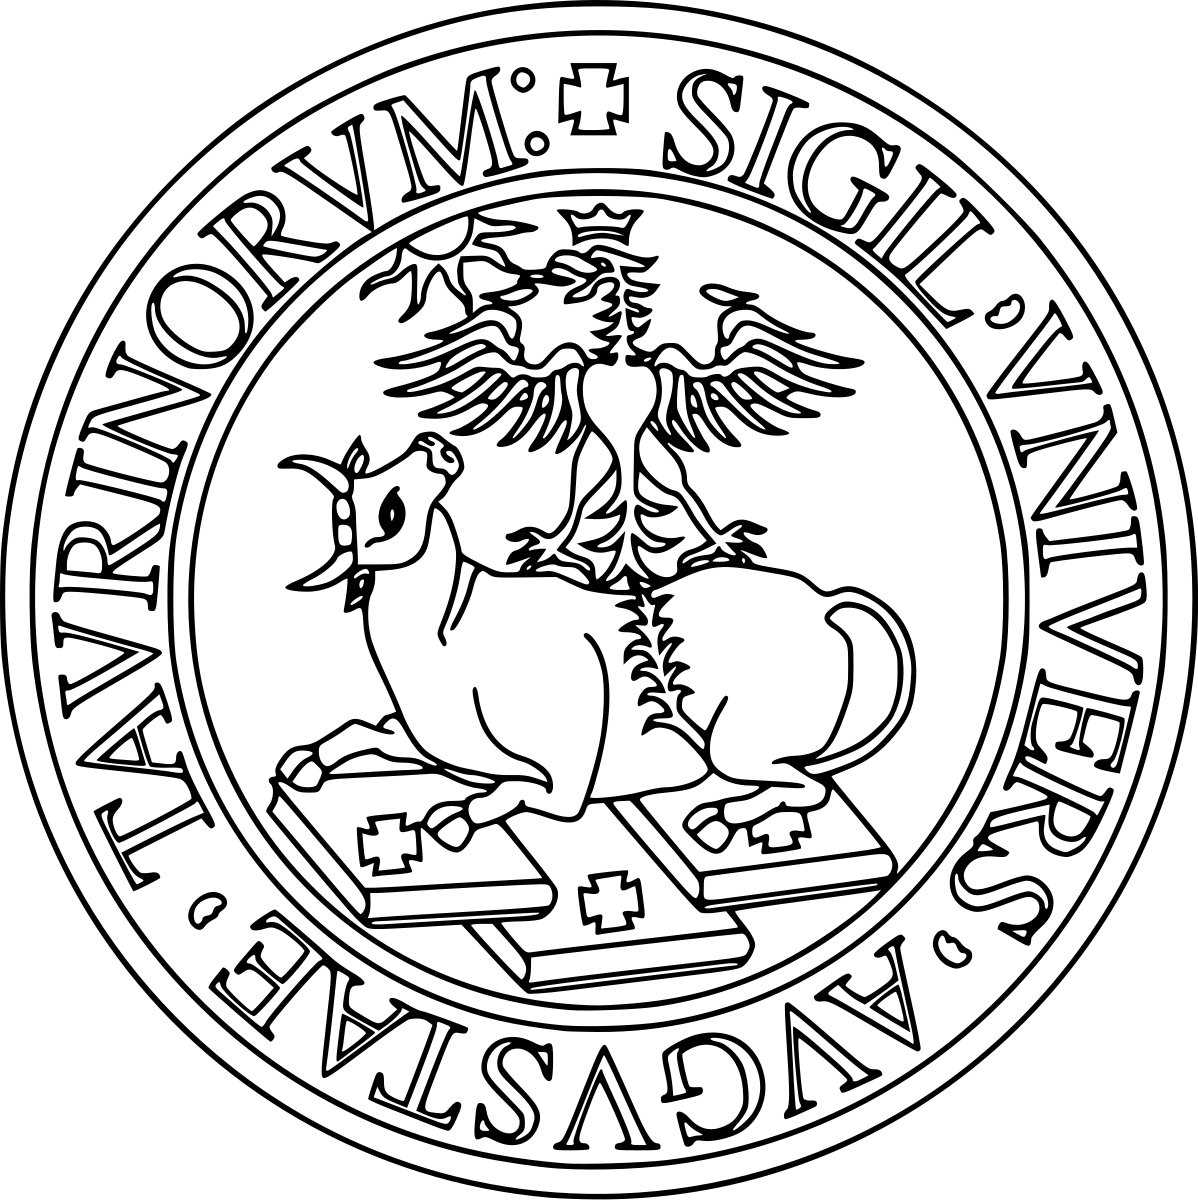
\includegraphics[scale=0.12]{Unito-logo} \\ \LARGE{UNIVERSIT\`{A} DEGLI STUDI DI TORINO} 
\\
TANS Course A.A. 2017/2018 Prof. Massimo Masera
\\
 \textbf{Ising Model Simulation with Monte Carlo methods}
}

\begin{document}
\date{}
\maketitle
\bigskip
\section*{Abstract}
In this work is introduced the Last Mile problem and the Agent-Based modelling process.
A solution for the Last Mile problem is proposed suggesting an active engagement of the population.
Some estimation has been done in order to make the simulation suitable for representing the city of Turin and actual cost of the delivering process.
Results show the robustness of the proposed solution both in economical and user's engagement terms, discussing also extreme situation.

%-----------------------------PAG 1----------------------------------%
\newpage
\section*{Introduction}
The Ising model is a well studied model in Statistical Mechanics which describes ferromagnetism phenomena. It is characterized by a microscopic configuration space based on D-dimensional lattice, that brings to macroscopic statistical quantities. Moreover it can easily generalize the concept of collective effects caused by binary valued points interacting in pairs; for this reason the Ising model became the core of the physics of complex systems. In the last decades computational methods have been applied to search a numerical solution for the 3D Ising model in order to  fill the lack of an analytical solution.  
\\
Alongside Metropolis algorithm became the most popular method of important sampling in MC. The basic idea of a weighted sampling based on the importance of a region determined a great step for the numerical solutions in general. Under these premises we want to outline the purpose this work wants to pursuit: finding numerical solution of the 3D-dimensional Ising model with Metropolis algorithm.


\begin{figure}[h!]
\centering
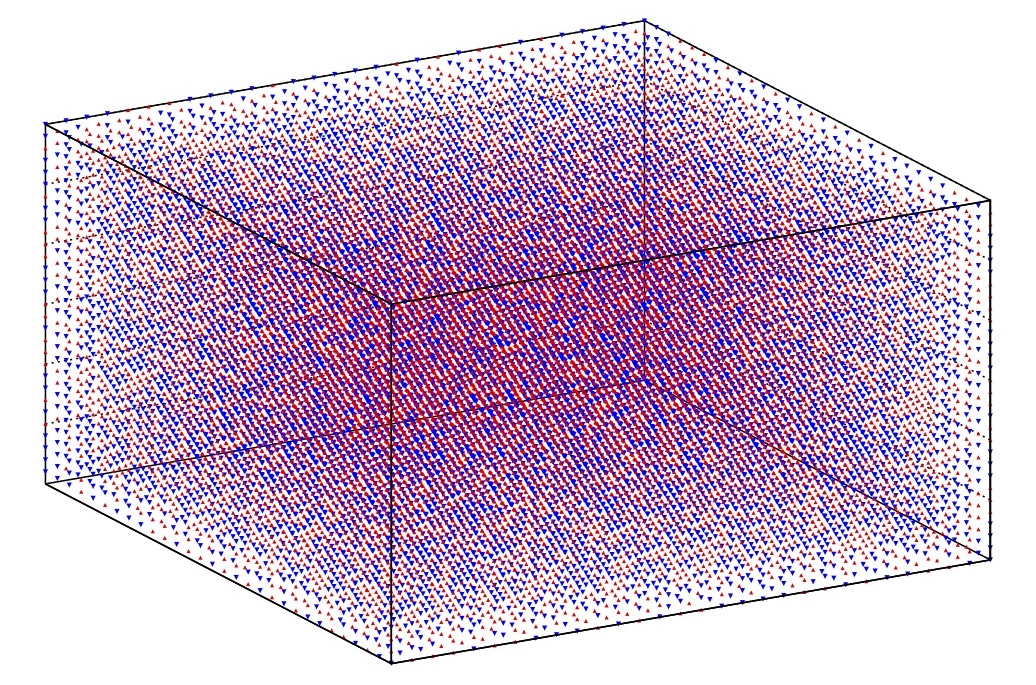
\includegraphics[scale=0.25]{img/img1_intro.jpg} 
\caption[Source: "monteinsing code" https://inknos.github.io/monteising/]{High temperature simulation of 3D Ising model}
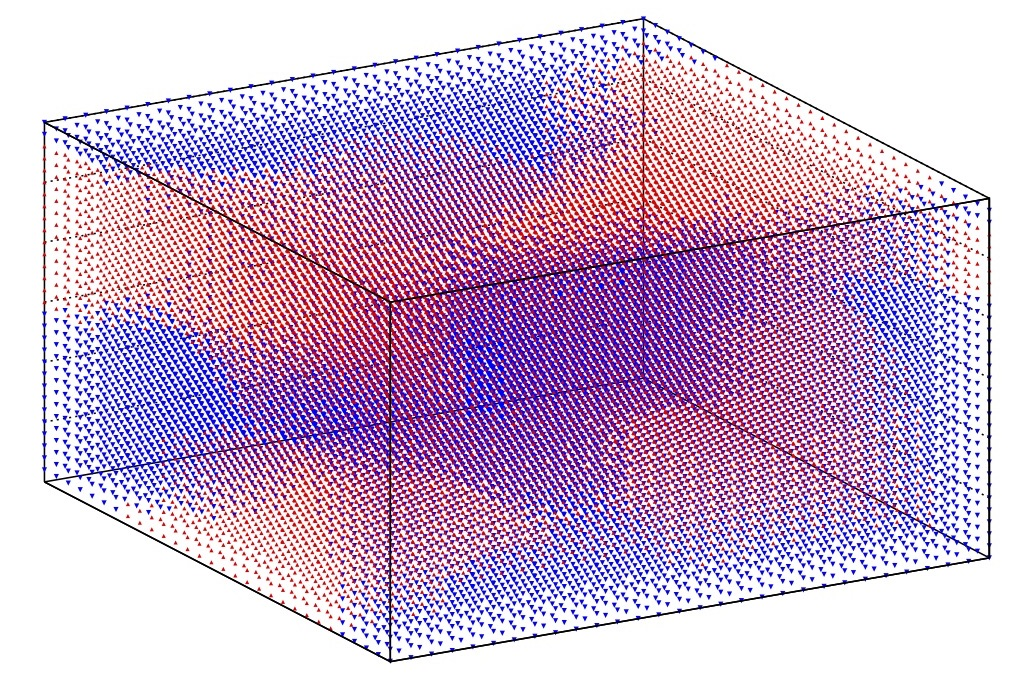
\includegraphics[scale=0.25]{img/img2_intro.jpg} 
\caption[Source: "monteinsing code" https://inknos.github.io/monteising/]{Low temperature simulation of 3D Ising model}
\end{figure}


%-----------------------------PAG 2----------------------------------%
\newpage 
\section{Theory}
\subsection{Ising model}
The Ising model is a physical-mathematical model which \\
The history of Agent Based Model can be traced back to 1940s and the Von Neumann cellular automata, a theoretical machine capable of self-reproduction following simple rules.
In the 1970s and 1980s we see the birth of Thomas Shelling's segregation model and Robert Axelrod's tournament of Prisoner's Dilemma algorithms.
By the 1990s, with the creation of NetLogo and Swarm software, the agent-based approach became widespread in social science and study of complex system.

An agent-based model (ABM) is one of a class of computational models based on the Agent-oriented programming (AOP), which simulates the actions and interactions of autonomous agents with a view to assessing their effects on the system as a whole. 
In other words the ABM's aim is to re-create and predict the appearance of complex phenomena simulating operations and interactions of multiple agents, only defining them and not the phenomena; the analogy to statistical mechanics is to define the system through its micro-scale details and then study the complex macrostate. 

Combining elements of complex systems, computational sociology, multi-agent systems and Monte Carlo methods (to introduce randomness) the complex behavior emerges from the lower (micro) level of systems, i.e. simple behavioral rules, to a higher (macro) level. 
This principle, known as K.I.S.S. (“Keep it simple, stupid")\footnote{Wikipedia: https://en.wikipedia.org/wiki/Agent-based\_model}, is extensively adopted in the modeling community. Individual agents are typically characterized as boundedly rational, i.e. they act pursuing their own interests, but from the point of view of an external observer they express heuristic decision-making rules, learning and adaptation that can be synthesized as: “the whole is greater than the sum of the parts", in the sense that we get more information than those we put in the system.

From a theoretical point of view there are three central concepts that distinguish ABM from other computational model. 
\begin{itemize}
\item \textbf{[Emergence]}The Agent-based model explore the complex system equilibrium deriving from simple rules of the agents instead of studying the system's equilibrium.
\item \textbf{[Agent-Object]} Agent-base models consist of dynamically interacting rule-based agents which can create a real-world-like complexity. 
Agents are typically situated in space and time, and their location and behavior are encoded in algorithmic form in computer programs. 
In some cases, though not always, the agents may be considered as intelligent and purposeful.
\item \textbf{[Complexity]} ABMs complement traditional analytic methods in the sense that the last characterize the equilibria of a system, while the first  allow the possibility of generating those equilibria. 
Agent-based models can explain the emergence of higher-order patterns and non-linear systems for which we do not have an analytic solution or the numerical one is too expensive from a computational point of view.
\end{itemize}

%-----------------------------PAG 3----------------------------------%
\newpage
\begin{figure}[h!]
\centering
%\includegraphics[scale=0.5]{ABM_segregation.png}   
\caption{Thomas Shelling's Segregation model (1978); Micromotives and Macrobehavior; New York: Norton. \\
Wilensky, U. (1997). NetLogo Segregation model. http://ccl.northwestern.edu/netlogo/models/Segregation. Center for Connected Learning and Computer-Based Modeling, Northwestern University, Evanston, IL.\\
Wilensky, U. (1999). NetLogo. http://ccl.northwestern.edu/netlogo/. Center for Connected Learning and Computer-Based Modeling, Northwestern University, Evanston, IL}
\end{figure}
 
\subsection{Monte Carlo methods and Metropolis algorithm}
In order to try solve the Last Mile Problem with an ABM, we have to forget the classical and analytical approach that involve finding a system of equation to be solved either exactly or numerically as a whole.

Instead each agent will act independently and the commissioner of the shipping will be only responsible of optimizing the cost, finding which agent can perform the task at the lowest price.
Unpacking the problem in such way it can be easily translate in terms of agent-based programming, indeed we can define a set of behavioral rules which bring the model to an overall stability situation through agent interactions.
However, as we said before, the solution independently emerges thanks to the computational representation of the problem complexity. 

Generally speaking, each courier can be seen as an instance of a class of agents which have as objective to minimize the journey and get much money as possible; on the other hand we have to define the environment where the agent can move, it could be as complex as a city or only a cartesian coordinate system.



%-----------------------------PAG 4----------------------------------%
\newpage
\subsection{NetLogo}
\begin{figure}[h!]
\centering
%\includegraphics[scale=0.31]{Figura2}  
%\caption[Source: https://ccl.northwestern.edu/netlogo/]
\end{figure}
NetLogo is a multi-agent programmable modeling environment. 
It is used by tens of thousands students, teachers and researchers worldwide, it powers HubNet participatory simulations, is authored by Uri Wilensky and developed at the CCL.\footnote{NetLogo website: https://ccl.northwestern.edu/netlogo/} 
NetLogo was designed in order to teach children the programming concepts using agents in the form of turtles, patches, links and observer. 
The variegate audience brought this language to be used in many scientific published articles.
NetLogo allows to explore emergent phenomena with a graphics interface consisting of switches, sliders, choosers, inputs, and other human-friendly interfaces, it has an extensive model library including models in various of domains, such as economics, biology, physics, chemistry, psychology, system dynamics allowing the user to create new models and modify the existing ones. 

BehaviorSearch\footnote{Behavior Search website: http://www.behaviorsearch.org} is a software tool to help automating the exploration of agent-based models (ABMs), by using genetic algorithms and other heuristic techniques to search the parameter-space. 
It interfaces with the popular NetLogo ABM development platform, to provide a low-threshold way to search for combinations of model parameter settings that will result in a specified target behavior. 
The model's parameters space exploration act in four steps:
\begin{center}
\framebox[14cm]{%
 \begin{minipage}{142mm}
 \begin{enumerate}
 \item Design a quantitative measure of the behavior you are interested in.
 \item Choose parameters to vary and the ranges are allowed into.
 \item Choose a search algorithm and run it.
 \item Examine the results (what parameters most affect the chosen       behavior?)
 \end{enumerate}
 \end{minipage}}
 \end{center}
\bigskip
In this work we used NetLogo 6.0 and Behaviour Search 6.0.

%-----------------------------PAG 5----------------------------------%
\newpage 
\section{Code}
This section's aim to introduce a possible solution to the Last Mile Problem that we investigated and modeled. 
The approach to this problem comes from the analysis of the city of Turin, in particular about the urban situation and the world of the sharing economy. 
First of all, as we shown in the introducing section, nowadays every city in the world is growing and becoming (in our terms) more complex, our case study will be Turin. 
This complexity causes inefficiency of transportation in urban area, the lack of mobility, and an increase of pollution. 
All forecasts about those problems  affecting cities are not optimistic and a lot of research is focused on this aspect. 
Starting from those premises we turn our interest on the world of sharing economy watching to:
\begin{center}
\begin{itemize}
\item BlaBlaCar (cars)
\item Enjoy (cars)
\item TOBike (bikes)
\item Foodora (bikes)
\end{itemize}
\end{center}
In particular there are 116 TOBike stations with about 10 bikes for each station and 186 Enjoy's cars in Turin. 
Morover there is 1 subway, 10 trams routes and 112 bus routes used by about 1200 vehicles; adding all the private vehicles for a population of 887,101 citizens we discover a great complexity about the transportation system in Turin. 

The main innovation of our idea is to convert this problem in our solution, finding a way to delivery goods all around the city increasing the efficiency as the complexity of a city grows. 
Basic idea is to deal with the delivery process by entrusting the last mile of the package's journey to people that are moving in town to their destination; this lays the bases for the inclusion of citizens, and their urban movements, in the transportation process transmuting them from passive user to active actor and ensuring the ecology of the process. 

We create a model that simulates people traveling with different vehicles in a space to their destination; each one could change his journey, diverting from the original one, in order to deliver a pack to its destination. 
Every person has a different “inner'' cost that depends on his vehicle and personal interest, this brings to an auction in which the delivery company aim at minimizing the expenses, corresponding to the product of the inner cost and the length of the deviation. 
In order to have a more efficient transportation, packs are located in different magazines in the space, taking inspiration to the 20 Amazon's lockers in Turin; obviously they are put in the nearest magazine to the pack's destination. 
The proportionality between deviation and expense needs an incentives analysis in order to reconcile the minimization of the company and the maximization of the ordinary citizen's benefits while guaranteeing the overall ecological benefits to the city.

\newpage
\subsection{Calibrating the model}
We aim at creating a simulation suitable for the chosen context, the city of Turin.

First we have to estimate the number of possible users interest in participating in a gig-economy-like project, so we analyzed the number of users of EnJoy, a nation-wide car-sharing service. these are roughly 5'000'000 in Italy, the 8\% of the population. Being almost 900'000 the citizen of Turin, estimating a similar percentage of people willing to engage in our project, we end up with 7000 possible candidate. For the purpose of our simulation we will scale down this number to 700, in order to contain the computation cost of the simulation.

Then we have to estimate the number of packs delivered in our city daily. We base our calculation on the number of packs delivered yearly by Amazon Inc., roughly 5'200'000 packs for the city of Turin alone, meaning about 14'000 packs delivered daily, supposing a uniform distribution all year along\footnote{Amazon Innovation Awards 2017, University of Turin, Torino}. Again for the sake of computational cost we will scale this number to 1'400, consistently with the proportion used before.

Considering that Amazon charges approximately 6\euro{} for a “same-day" pack delivery and the last mile's contribution to the entire journey cost (from producer to customer) is about 30\%, we defined a maximum threshold of 1.75\euro{} for the simulated delivery.

As for the cost of the basic infrastructure needed, namely a number of short-term deposit in which packages are stored around the city, we set 700\euro{}/month the cost for a 24sqm room, comprehensive of maintenance, rent ad basic bills. This scales to about 3\euro{}/month for a 50x40x30cm box, about 0.2\euro{}/pack for a permanence of two days. Fixed cost are considered negligible in the context of our simulation, being considered as long-term investment.

Lastly we have to map the size of the city to the patch-size of our model. Turin is roughly 12km radius, a distance that can be covered on average\footnote{35mins by car, 150mins by foot} in 75 minutes. This means that the length of a workday, from 8.30 am to 9.00 pm, being 1 patch/tick the speed of our agents, will be such that each agent is capable of going back and forth from one end to the city to the other about 10 times a day; being the radius of our city proportional to the map's diagonal. This can be translate in NetLogo's language assuming 1600 ticks equals a day.

%-----------------------------PAG 6----------------------------------%
\newpage 
\section{Code}
The basic idea of this work is to give the possibility to every one is traveling in the city to transport a pack to its destination. 
This is a simple concept that, as we shown in the previous section, has some implications. In order to introduce the code to the reader it is useful to present the simulation through its evolution, i.e. we want to show how the code has changed starting from the first idea/solution for the Last Mile Problem to its generalization. 
We remind that the code is written in NetLogo 6.0 and it is possible to freely download it and run the simulation.


\subsection{Moving agents in a cartesian coordinate system}
First of all we have to implement a code that simulates the movement of a defined number of agents in a environment characterized by an empty cartesian coordinate system. 

\begin{figure}[h!]
\centering
%\includegraphics[scale=0.44]{3_1}  
\caption{Moving agents and fixed storages}
\end{figure}

\subsubsection*{Basic Agents}
The basic agent in our simulation will be a breed called “user" moving freely.
They will have a set of own variable, at this point only the destination.
Agents are created in random patches ad are assigned other random patches as destination.
Each agent will then move toward their destination in a straight line and die once reached it.
To avoid the extinction of users, a new one is created in the patch the previous one died.

\subsubsection*{Special Patches}
A special patchset is created to represent the storages around the city.
These patches will be identified by a boolean value, indicating the role of storage or not, and, if so, they will also own a variable “space", that will be further used to represent the physical space in a storage room.
\looseness=-1

\newpage
\subsection{Moving packs}
Once create the basic structure we need to simulate the transportation of packages around the city done by users.
\medskip
\begin{figure}[h!]
\centering
%\includegraphics[scale=0.5]{3_2}  
\caption{Agents delivering packs}
\end{figure}
\medskip
\subsubsection*{Packages}
A breed called “packages" is created in order to simulate the goods transported in the space. Each package will own two variable, one for the destination and another, boolean, to indicate if they are assigned to a user or not.
Each packages is placed in a locker-patch ad assigned a random point on the map as destination.

\medskip
\subsubsection*{Pick-up}
In order to be picked up a package needs to be put in relation with a user.
At first this will be done randomly, the user will go from his position to the position of the package, then do the destination of the package and lastly to his own destination.
To properly keep track of what a user is doing we need to add two new variables to the user breed, “busy" and “bag". Bag will contain the id of the assigned pack and busy will be true if the pack is being transported to its destination by the user.

\newpage
\subsection{Optimizing}
Since now all operation are done randomly and with no regards to the optimization of the process. We need to introduce a way to properly choose the package-user couple such that the distance traveled is minimal.

\begin{figure}[h!]
\centering
%\includegraphics[scale=0.39]{3_3}  
\caption{Cost evolution after auction}
\end{figure}
\subsubsection*{Auction}
To optimize the travel we will use an auction for each package.
Each user will have a new variable, “cost", that will be the amount of a virtual money needed to be paid in order to deviate one patch off the straight line connecting the origin and the destination of the user.
Each package will ask all the user the amount they will need in order to deviate from their original route, pick them up and bring them to destination: the lower bidder will be assigned the pack and will proceed with the delivery.
\begin{figure}[h!]
\centering
%\includegraphics[scale=0.45]{auction}  
\end{figure}
\looseness=-1
\newpage
\subsection{Making it real}
At this point we already have all the essential part of our simulation: agent moving around, delivering packs, in a sort of optimized process. Yet we are far from real and some elements need to be taken into account.

\begin{figure}[h!]
\centering
%\includegraphics[scale=0.4]{3_4}  
\caption{Complex movement behaviour}
\end{figure}
\medskip
\subsubsection*{Highest cost}
The commissioner will not be willing to pay any amount to have his packages delivered, a maximum cost per package is fixed, if the lowest bidder ask for a total amount higher than the fixed maximum cost, the package is not assigned and the auction run again.
\medskip
\subsubsection*{Goods placement}
Packages are not placed randomly in the storages patches but, if the space is enough, each package will be placed in the storage nearest to its destination.

\begin{figure}[h!]
\centering
%\includegraphics[scale=0.77]{place_pack}  
\end{figure}
\newpage
\subsubsection*{Day and night}
People fluxes are not constant during the day, in a city they follow the home-work path one way or the other in the morning and in the evening.
To simulate that we suppose that after a certain amount of ticks we switch from morning to evening.
The cartesian space is divided in two section, the left and the right one respectively along the xcor, during one part of the day agent will be assigned a destination on one side with an higher probability, the other way round during the other part of the day.

\begin{figure}[h!]
\centering
%\includegraphics[scale=0.8]{dest_day_night}  
\end{figure}

\subsubsection*{Randomness}
Random behaviour are created for user: they may, with a small probability, not accept to deliver a package, their internal cost is uniformly distributed around a mean value instead of being fixed.

\subsubsection*{Maintenance cost}
As we can expect the maintenance of all storages around the city will have a cost, more and bigger storages will cost more and add up to the expenses of the commissioner. A value can be chosen to simulate this cost.

\subsection{City of Turin}
In order to scale the simulation to the city of Turin, a series of metric are calculated with the same ratio we can find in the real life, as explained in the previous chapter.

\begin{figure}[h!]
\centering
%\includegraphics[scale=0.8]{scaling}  
\end{figure}

\newpage
\section{Results}
In this section we present the results obtained from the Agent-Based simulation. We discovered that the solution is feasible i.e. people traveling in the city can deliver all packs on time and with a total expense that is lower than the upper-bound (1.75\euro{} per pack). Moreover, being the Foodora's employee salary about 0.5\euro{}/km, we can see that in our estimated range of parameters a person can be paid more than a common delivery man.

Using genetic algorithms implemented in Behavior Search 6.0 we optimized the number of storages and their space, keeping all other estimated parameters fixed such as the number of users, the number of packs and the cost of each box in the storage. 

Figure below show the fitness minimization (expenses) with the following parameters: 1400 packs, 700 users, 1\euro{}/km for users' deviation, 1.75\euro{} as maximum expense for a pack delivery, 0.2\euro{} cost storage's box.

\begin{figure}[h!]
\centering
%\includegraphics[scale=0.33]{BS-02lcost-10lmax-lspace304} 
\caption{Behavior Search result: 10 storages with 304 boxes each, total expense 1439.28}
\end{figure}

Considering 0.8\euro{} as storage's box cost, we find again that the number of boxes in each storage is greater than the minimum needed. This implies that spending money for having bigger storage is useful in case a pack has to be delivered in the neighborhood.

\begin{figure}[h!]
\centering
%\includegraphics[scale=0.33]{BS-08lcost-10lmax-153lspace.png} 
\caption{Behavior Search result: 10 storages with 153 boxes each, total expense 1542.02}
\end{figure}

\newpage 
May be found interesting for the reader to have a deeper look at two of the most important curves in our simulation: number packs vs. time and total expenses vs. time. 

The figure below show that the number of packs exponentially decreases with time as expected.

\begin{figure}[h!]
\centering
%\includegraphics[scale=0.59]{Grafici/Packs(02lcost_10lmax_304lspace).png} 
\caption{Numb packs vs. ticks (10 storages with 304 boxes each, 1400 packs, 700 users)}
\end{figure}

In order to roughly estimate the curve decrease we did a linear regression with 0.07 mean squared error.

\begin{figure}[h!]
\centering
%\includegraphics[scale=0.59]{Grafici/Packs(02lcost_10lmax_304lspace)[E_0,07].png} 
\caption{Fit: numb packs vs. ticks (10 storages with 304 boxes each, 1400 packs, 700 users)}
\end{figure}

\newpage
On the other hand the total expenses approximately increase as a logarithm, which compensates the number of packs trend.

\begin{figure}[h!]
\centering
%\includegraphics[scale=0.6]{Grafici/Total_expense(02lcost_10lmax_304lspace).png}  
\caption{Total expenses vs. ticks (10 storages with 304 boxes each, 1400 packs, 700 users)}
\end{figure}

Even if the mean squared error is considerably worse than the first fitting, we can have an estimate of the curve slope.

\begin{figure}[h!]
\centering
%\includegraphics[scale=0.6]{Grafici/Total_expense(02lcost_10lmax_304lspace)[E_4272].png}  
\caption{Fit: total expenses vs. ticks (10 storages with 304 boxes each, 1400 packs, 700 users)}
\end{figure}

\newpage
At any instant we have a different average cost of delivery, so we can plot the ratio between expenses and packs vs. time. As shown in the figure below the initial costs are relevant but they decrease rapidly with time.

\begin{figure}[h!]
\centering
%\includegraphics[scale=0.8]{Grafici/Total_expense_Packs(02lcost_10lmax_304lspace).png}   
\caption{Total expenses/numb packs vs. ticks (10 storages with 304 boxes each, 1400 packs, 700 users)}
\end{figure}
 
\newpage
\section{Extreme Cases}
As a proof of concept we decided to analyze some extreme cases in order to explore if our solution is robust enough to survive real-life challenges.

\subsubsection*{Too few}
What would happen if there are too few users? 
Keeping all other parameters as found we set the number of users to one tenth the original value, down to 70 agents total.
We observe that the delivery process takes up to two days, instead of the half day in standard situation and the total expenses increase up to 28\% more.



We can have an estimate of the curve slope in log-lin scale.



\newpage
\subsubsection*{Too many}
On the opposite we explore what happens if there are too many users, up to 7000 agents total.
As can be expected the delivery process is completed in a risible time and the expenses are down 70\%, proving the benefit for the commissioner in expanding the participation.


We can have an estimate of the curve slope in log-lin scale.



\newpage
\subsubsection*{Wanting more}
A reasonable question may that an higher pay may be needed to incentive users to participate in the activity. 
We examined what would happen if the pay was up to 5\euro{}/km of deviation.
Similarly to the first case, the process of delivering all packs may take up to two days, but the total expenses will not be too different than the standard situation.


We can have an estimate of the curve slope in log-lin scale.



\newpage
\subsubsection*{High Maintenance}
A success of our method may have the downside of increasing maintenance costs for the storages around the city.
Examining a bi-daily maintenance cost five time the standard situation we found an increase in the total expenses around 21\%, like the first case examined, but without any other downside.



We can have an estimate of the curve slope in log-lin scale.



\newpage
\section{Conclusions}
This work has analyzed a new solution for the LMP characterized by the delivery process carried out by citizens. As we shown in the first section, the today city complexity brought a proportional increase of the transportation costs in it; indeed the presented solution, based on the sharing economy, can be ecologically and economically sustainable. Citizen becomes active actors in the transportation process delivering packs all around the city. The Agent-Based Model has been realized with a scaled map in order to express the Turin's distances and adequate (from a computational point of view) parameters: 
\begin{center}
\begin{tabular}{c|c|c|c|c}
 \hline 
 Numb. Packs & Numb. Users & Max Delivery Cost & Storage Box Cost & Users' Pay \\ 
 \hline 
 \hline
 1400 & 700 & 1.75 \euro{} & 0.2 \euro{}/two days & 1 \euro{}/km \\ 
 \hline 
\end{tabular} 
\end{center} 
The code has been written in NetLogo 6.0 and, thanks to the Behavior Search tool, brought the following results for parameters we need in order to minimize the expenses: 
\begin{center}
\framebox[12cm]{%
 \begin{minipage}{100mm}
 \begin{itemize}
 \item 10 Storages.
 \item 304 Boxes in each storage.
 \item Total expenses: 1440 \euro{}
 \end{itemize}
 \end{minipage}}
 \end{center}
Note that the storage's capacity is greater than the minimum required for an uniform distribution of 1400 packs in 10 storages. This shows how the complex system achieves a store optimization for minimizing the expense regarding random place of delivery.
\bigskip

The figure below shows that the curves of expenses and number of packs vs. time have almost an opposite trend; moreover on the right we see that the expenses for each pack decreases with time.

\newpage
Considering an high and a low number of users we saw that the convergence is faster in the first case and, as expected, less expensive. Note that at the end of the day (1600 ticks) in both cases all packs are delivered.


Increasing the fixed cost parameters we saw that expenses grew, but the model still succeed in delivering all packs in a day (1600 ticks) with a cost for each pack that is lower than 1.75\euro{}.
\\
In conclusion this underlines the robustness of the proposed solution both in economical and user's engagement terms, moreover the model held interesting results also in extreme cases. 

\subsection*{Further development}
The model could be extended by considering:
\begin{itemize}
\item improved economic model;
\item GIS map of the city of Turin;
\item daily data for a real time calculation.
\end{itemize}
\end{document}
